% !TEX root = main.tex
\section{Conceptualization for Relationship Explanation}
\label{sec:conceptualization}
In this section, we give our solution to compute $P(c|e_i)$, the probability that $c$ is a concept of entity $e_i$.
We use Probase, a web-scale taxonomy, for the computation. We first briefly introduce Probase and give a direct solution. However, the direct conceptualization solution ignores the unique setting of relationship explanation. We will analyze the problems caused by our problem setting then give an improved version.problem here is that 

\subsection{Problem Statement}

\yh{intro about probase, copy from xiangyan's paper}

Given an entity $e$, from Probase, we can acquire its concepts' set $C(e)$. For each $c_i \in C$, the frequency $n(c_i,e)$ can be accordingly derived, which means how many times the $e$ isA $c$ can be observed from the corpus. The frequency information allows us to estimate  $P(c|e)$ by 
$$P(c|e)=\frac{n(c,e)}{\sum_{c_i\in C(e)}n(c_i, e)}$$


\paragraph{Refinement by Head Concepts}
We further argue that the relationship between entities are determined by the head concepts. For example, the \at{founder} relationship between \at{Apple Inc.} and \at{Steve Jobs} are determined by the head concepts they possessed (e.g.\ \term{company} and \term{entrepreneur}, regardless of the modifiers such as \term{technology} in the concept \term{technology company}.) Hence, the attribute should be generated by the head concept pair instead of the concept pairs with modifiers. This motivates us to refine the optimization objective by summing over on the head concept pairs. Let $\bar{C}_1$ and $\bar{C}_2$ be the head concepts in  $C_1$ and $C_2$, respectively. Our problem is refined as:
\begin{equation}
\label{eq:target}
\argmax_a \sum_{c_i\in \bar{C}_1 , c_j \in \bar{C}_2 }P(a|<c_{i},c_{j}>)\times P(<c_{i},c_{j}>|<e_{1},e_{2}>),
\end{equation}

By restricting the concept to the head concept, we can further reduce the computation cost.
The number of head concept pairs is obviously significantly smaller than that of the concept pair and that of entity pairs. Because most concepts are tail concepts with long modifiers. Head concept allows us to find the limited number of relationships without handling the huge number of long-tailed concepts and their entities. 

\paragraph{Conceptualization into Head Concepts}

Given a head concept $c_h$, we need to estimate $p(c_h|e)$. However, we are likely underestimate $p(c_h|e)$ because in genereal there is no sufficient direct isA relationships from entity $e$ to the head concept $c_h$. We illustrate this in Example~\ref{exa:conc}. For our task, we only need relatively general concepts(a.k.a. head concepts).
\begin{example}[Underestimation of head concept]
\label{exa:conc}
Consider the entity \ac{Mona Lisa}. Its concepts in Probase include \ac{\{painting, famous painting, world's most famous painting\}}. The frequency between \ac{Mona Lisa} and each concept are\term{33,8,1}, respectively. The isA link from \at{Mona Lisa} and \ac{Painting} is missing since we always talk about \at{Mona Lisa} as a famous painting. Directly using the data in Probase, we have $$P(\ac{Painting}|\at{\text{Mona Lisa}})=0$$, which is obviously an underestimation. 
\end{example}


For each entity $e$, we first retrieve all concepts of $e$ in Probase. Let the set of these concepts be $C(e)$. Then, we reduce $C(e)$ to $\bar{C}(e)$ so that each concept in $\bar{C}(e)$ contains all head concepts of each concept in $C(e)$. \yh{We identify the head concept by ... .}. We denote each head concept as $c_h$ and the concept with modifiers as $c_{l}$ are the rest. Our problem is reduced to the recalculation of the probability $P({c_h}|e)$.
\yh{in experiments, we should compare the baseline that directly use concepts instead of head concepts.}



\begin{example}[Head concepts VS Original concepts]
\label{exa:HvsO}
Take \term{famous painting} as example. Its original concepts are \term{image, treasure}, which are reasonable but not plausible, since their occurrence are 2 and 1 respectively. However, the most plausible concept \term{painting} is not among the concepts.
\end{example}

\yh{Rewrite the objective function when we only consider the head concepts}

\paragraph{The main steps}
Given an entity $e$ from $Probase$, we can get its concepts from probase. First we do head modifier detection based on syntax[], since the concepts in Probase all follows English grammar, this approach already produces a good result. Next, we recalculate the probability of $P({c_h}|e)$ by aggregating the contribution from $c_l$. The essentiality of doing so is illustrated in Example~\ref{exa:recalc}. Finally, we provide a method to take the original isA relation from Probase into consideration.




\begin{example}[Essentiality of Aggregation]
\label{exa:recalc}
\term{steve jobs} The concept\term{well-known name} has four occurrences however \term{name} has only 2. There are other modifiers for the same head, so that the typicality of the head will be largely underestimated.
\end{example}



\subsection{Baseline}

The basic idea of the improved estimation is aggregating the information of all subconcepts of the head concepts.  We should contribute all the counts of $C_{l}$ to $C_{simple}$.


After head modifier detection, we have a set of ${c_h} \in C_{simple}$, among all the $c_{l_j}\in C_{l}$, there are 2 cases in the probase determined by whether the $c_{l_j}$ has an isA edge towards ${c_h}$ or not.
The intuition of doing so is illustrated in the Example~\ref{exa:clc}:

\begin{example}[contributing long concepts]
\label{exa:clc}
Assume that  \term{Mona Lisa is a painting} and \term{Mona Lisa is a famous painting} are observed respectively \term{33 times and 8 times} from different documents, we will get the knowledge that \term{Mona Lisa is a painting} occurs \term{41 times} instead of \term{33 times}.
\end{example}

Hence, the most straight forward approach is to contribute the corresponding long concepts to the simple ones as follows:

$$\hat{n}(c_h, e)={n}(c_h, e)+\sum_{ h(c_l)=c_h} n(c_l,e)$$
$$\hat{P}(c_h|e)=\frac{\hat{n}(c_h, e)}{\sum_{c_{h'}}{\hat{n}(c_{h'}}, e)}$$
where $f_{HM}()$ is a function that takes a long concept and produce a head concept.
....... Head concept space, typicality....
\yh{rewrite example}


\subsection{Combined Model with Original IsA}
When obtaining $\hat{P}(c_h|e)$, we are in fact judging the typicality of a concept.
In this section, we take the original Probase IsA relation into consideration. In Example.~\ref{exa:isagood}, we can observe some reasonable results produced by the Probase isA relationship.

\begin{example}[Resonable isA Relation]
\label{exa:isagood}
  There exists several original IsA concepts of the long concepts that are also reasonable. For example \term{ topaz}(a kind of yellow gemstone) has the concept \term{precious stones}, and \term{precious stones} has an edge towards \term{material} which is reasonable.
\end{example}

Based on the how to treate $c_l$, we have the following 2 cases:

\begin{description}
  \item[$c_l$ appear as an concept] In this case the counts that its entities produced should be take into consideration into $c_h$, deriving the following Case A.
  \item[$c_l$ appear as an instance] In this case $c_l$ is observed from the corpus as an instance at the left side of an isA sentence, it should be treated the same as other entities $e$, deriving the following Case B.
\end{description}


Therefore, to calculate  $P({c_h}|e)$, there are three cases.:

\begin{description}

\item[Case A.1 $e$ \isa ${c_h}$ ]
 The entity has has an isA edge towards one or more simple concept, which gives the original $P_{org}({c_h}|e)=$


\item[Case A.2 $e$ \isa $c_{l}$ \noisa ${c_h}$]  The solid edge here refers to the isA relationship in $Probase$ and the dashed one refers to the edge generated by head modifier detection. Example~\ref{exa:wahro} pointed out that there won't be necessarily an isA edge from \term{famous painting}($c_{l}$ ) to \term{painting}(${c_h}$), however $c_{l}$ is obviously a hyponym of ${c_h}$. In this case,
    % since it's detected by the head modifier method, we assume
    % $$P_{head}({c_h}|c_{l_j})=1 $$
    we have to re-calculate the $P({c_h}|{c_l})$.
    In the original probase approach, we use Eq.~\ref{phgl_org} to calculate the probability.
    \begin{equation}\label{phgl_org} P({c_h}|{c_l}) = \frac{n( {c_h},{c_l} )}{ \sum{n( {c_h}^*,{c_l} )}  } \end{equation}
    However, $n( {c_h},{c_l} )$ is lower than expected due to the reason demonstrated in Example.~\ref{exa:wahro}.
    Therefore, we alternatively utilize the $\sum{ e^*,n({c_l}) } $ as the occurrence of $c_l$, following the assumption that \em{ whether $c_l$ is typical towards its $c_h$ is independent from }
    $$P_{head}(c_h|e)=\frac{\sum_{c_h= f_{HM}(c_l*)} n(c_l*,e)}{ n(e)} $$

\item[Case B $e$ \isa $c_{l}$  \isa ${c_h}$]  In this case, we need to calculate the following equation
$$P({c_h}|e) = \sum_{c_{l}^*\in C_{l}}   P({c_h}|c_{l}^*,e)   \times    P(c_{l}^*|e) $$
, where $P(c_{l}^*|e)$ can be obtained from $Probase$ and
\begin{equation}P({c_h}|c_{l},e) = \frac{n({c_h},c_{l}, e)}{n({c_h}, e)}\label{eq:pcge}\end{equation}
We assume that the occurrence of $e$ does not affect $P({c_h}|c_{l})$ equivalently speaking, $P({c_h}|c_{l})$ is independent from $e$, thus Eq.~\ref{eq:pcge} can be simplified
$$P({c_h}|c_{l},e) =P_{probase}({c_h}|c_{l}) = \frac{n({c_h},c_{l})}{n({c_h})}$$
which can be obtained from $Probase$.

\end{description}

\begin{example}[Why aren't head relationship observed]\label{exa:wahro}
There are less chance of occurring \term{Famous painting is a painting} in the corpus, since human takes it for granted and will seldom express it in such a way, so that there won't be necessarily an isA edge from \term{famous painting} to \term{painting} in the KB, while we insist it is necessary.
\end{example}

%%%%%%%%%%%%%%%%%%%%%%%%%%%%%%%%%%
%\nop{
%In both case B.1 and B.2, the weight of the edge $c_{l}$ \isa ${c_h}$ is underestimated. We argue that when calculating the typicality $P({c_h}|e)$, the counts of the long concept contributing to its head concept should be re-estimated as follows.
%
%Notice that the boundary between case B.1 and case B.2 are not strict, there are such edges that have low observation in Example~\ref{exa:HvsO}. So that if we consider them as a whole, we can derive:
%\begin{equation} P({c_h}|c_{l})=\lambda P_{head}({c_h}|c_{l})+(1-\lambda)P_{probase}({c_h}|c_{l}) \label{eq:pcgclong}\end{equation}
%where $\lambda$ is a parameter \xch{principle: related to plausibility, number of occurrence, varies for different $c_{l}$ should it be derived from learning ?} since we assume $P_{head}({c_h}|c_{l})$ to be 1, Eq.~\ref{eq:pcgclong} is simplified to:
%$$P({c_h}|c_{l})=\lambda  +(1-\lambda)P_{probase}({c_h}|c_{l}) $$
%}
%%%%%%%%%%%%%%%%%%%%%%%%%%%%%%%%%%%%

Considering Case A.1 and Case A.2 we get the baseline. When calculating typicality, we should consider the both cases of $c_l$, thus combining Case A and B through a linear combination.

Finally  $P({c_h}|e)$ is calculated using the following equation:

\begin{equation}
\begin{split}
P({c_h}|e) = \alpha \hat{P}({c_h}|e)+ (1-\alpha) \sum_{ c_{l}^*\in C_{l} } [P({c_h}|c_{l}^*) ] \times  P(c_{l}^*|e)
\end{split}
\label{eq:pgge}\end{equation}






\begin{figure*}[!hptb]
\label{fig:pgge}
\centering
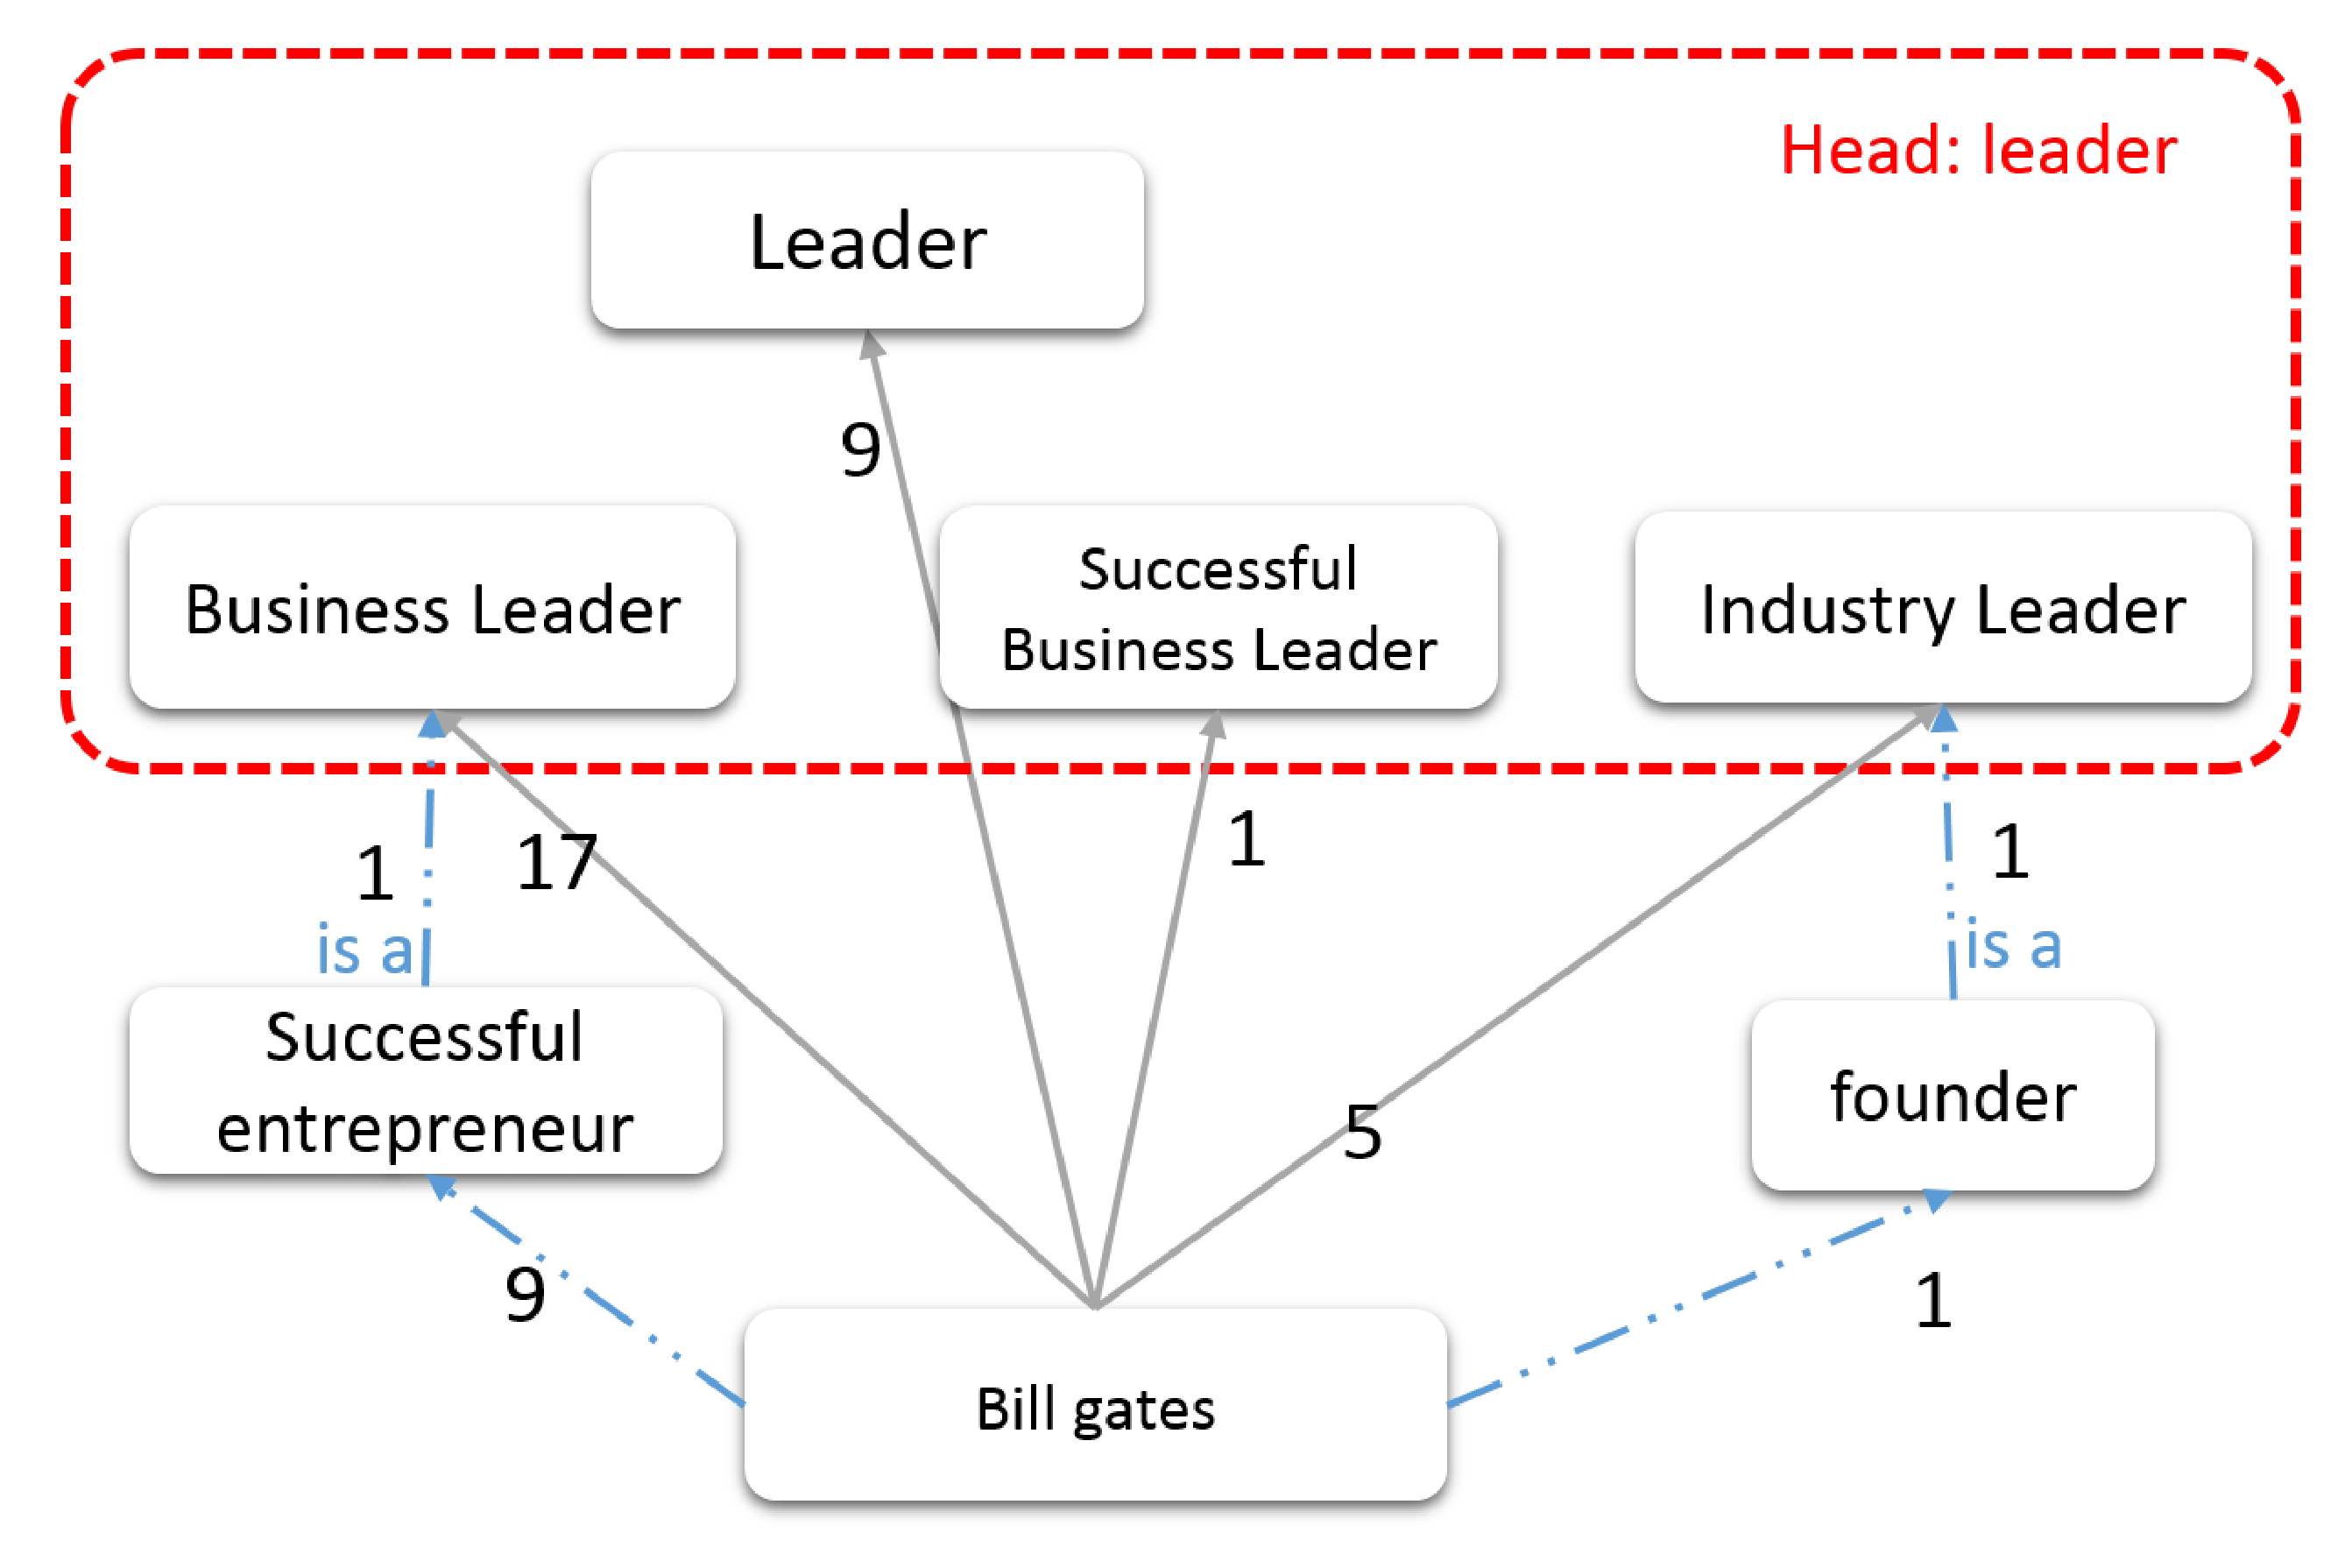
\epsfig{file=resources/bill_gates_isa.eps,width=5.5in}
\caption{calculating $P({c_h}|\term{Bill Gates})$ }
\end{figure*}


\nop{
\begin{tikzpicture}[->,>=stealth',shorten >=1pt,auto,node distance= 3 cm,
  thick,main node/.style={circle,fill=blue!10,draw,font=\sffamily\bfseries,align = center}]

  \node[main node] (4) {piece};
  \node[main node] (2) [left of=4] {painting};

  \node[main node] (5) [below of=2] {oil painting};
  \node[main node] (6) [left of=5] {famous\\painting};
  \node[main node] (7) [left of=6] {world's\\most famous\\painting};

  \node[main node] (10) [right of=5] {art piece};
  \node[main node] (11) [right of=10] {historical\\art piece};

  \node[main node] (12) [below of=6] {Mona lisa};


  \path[every node/.style={font=\sffamily\small}]

    (5) edge  node [left] {$\lambda_{i3}$} (2)
        edge [bend right] node [right] {\small{$ 0.65\alpha_{i3} $}} (2)
        edge  [bend right] node[left]  {\small{$ 0.28\alpha_{i3} $}} (4)
    (6) edge [bend left] node [right] {$\lambda_{i1}$} (2)
    (7) edge [bend left] node [right] {$\lambda_{i2}$} (2)

    (10) edge [bend right] node[right] {$\lambda_{i4}$} (4)
    (11) edge node[right] {$\lambda_{i5}$} (4)
    (12) edge [bend right]node[right] {0.01} (10)
         edge [bend right]node[right] {0.007} (11)
         edge node[right] {0.04} (5)
         edge node[right] {0.05} (6)
         edge node[right] {0.007} (7)
         edge node[left] {0.23} (2)
         edge [bend right]node[right] {0.04} (4);

\end{tikzpicture}
}


%
%The process of calculation is illustrated in the example~\ref{exa:calc}
%
%\begin{example}[Calculating $P({c_h}|e)$]
%\label{exa:calc}
%As illustrated in Fig.~\ref{fig:pgge}, the process of calculating the typicality a concept is as follows, where \term{painting} is ${c_h}$ and \term{Mona Lisa} is $e$. Then $P(\term{painting}|\term{Mona Lisa})$ consists of 2 parts, the direct edge $P_{original}({c_h}|e)= 0.23$, and the second part
%$$\sum_{ c_{l}^*\in C_{l} } [ \lambda_{i}^*+(\alpha_{i}^*) P({c_h}|c_{l}^*) ] \times  P(c_{l}^*|e) $$
%$(\alpha_i^*+{c_h}^*=1)$
%Thus we get
%$$ P = 0.007\times \lambda_{i2}+0.05\times \lambda_{i1}+0.04\times(\lambda_{i3}+0.65\alpha_{i3}) $$
%For \term{piece}, it is the similar process. The relation here is only part of the whole graph.
%\end{example}




We consider only 2 layers of isA relationship for 2 reasons. The first one is that more layers will lead to noisy concepts such as \term{issue, factor, element}, which are concepts for almost eveything, Secondly, discussing the transitive relation between concepts is beyond the scope of this paper.
